\subsection{Methodology}
It is essential that the methodology of the evaluation for the product-test is defined. To achieve this, the desired outcome of the test must be clearly identified i.e. a proper strategy for evaluating whether or not, and to what degree, the final problem statement has been answered. Furthermore, the relevance of the established list of requirements must be tested.

The main criterion of the product test can be defined thus in bullet points:
\begin{itemize}
\item To investigate whether or not the final problem statement has been answered.
\item To prove/disprove the relevance of the list of requirements.
\end{itemize}

\subsubsection{Qualitative / Quantitative }
In order to conduct a proper test one must decide which technique that must be used in terms of the gathered data. Quantitative data can easily be translated into measurable data elements for ex. Magnitude, amount, size etc \parencite{Rogers2002}.

Qualitative data is the data expressed in form of themes, patterns and expressions \parencite{Rogers2002}, being the data which can be interpreted such as opinions, descriptions and observations.

In order to proper evaluate the product, it can arguably be plausible, that by utilizing both qualitative and quantitative data acquiring methods, a triangulation of verified data is acquired.

\subsubsection{Approach} \label{sec:approach}
In accordance with the final problem statement, we can establish that it is of little relevance to study the human relations. Due to the fact that some strict boundaries has been established for the parameters of the problem statement i.e. whether the constructed controller can be comparable to SOTA-controllers in terms of functionality, it can be concluded that the main objective is to validate a balanced comparison. 
\bigskip

\textit{"Often, there isn’t a clear, well-defined population of potential respondents. There isn’t a list or a central repository of people that meet a certain qualification and could be respondents. That may just be the nature of the population. So strict random sampling cannot be done. However, valid data can still be collected through non-probability-based samples."} \parencite{Lazar2010}
\bigskip

As Jonathan Lazar (et al) argues in Research Methods in Human-Computer Interaction, valid data can be obtained from a non-probabilistic based research method, and given no well-defined target group other than people with an interest in vehicle-games, it is assumable a durable solution to a testing-framework.
Since the objective of the project is not self-explanatory and the chosen alternative way of controlling a vehicle based game, some measure of introduction is required. Therefore it is advisable that methods such as field-observation with a complete observer basis are avoided. 	


\subsubsection{Hypothesis vs. theory} \label{sec:hypotheory}
When determining the experiment structure, it can be of great significance to first create an overview regarding goals, and what is essentially important to learn from a product-test. Without such goals, a product test might ultimately be rendered futile.
\bigskip

In the book Research Methods in Human-Computer Interaction, it is argue that an experimental design depends on whether it is a theory or a hypothesis that needs to be tested. A theory usually requires a more thorough study and additional experiments to either prove or disprove. The problem statement in this report, and the structure as of whole is more close to a hypothesis, since it is asked whether or not a controller can be constructed, and it is hypothesized that the list of requirements  will increase the probability of a positive outcome i.e. they are required to establish a functional product. Hence it is assumed that an experimental structure baring similarities to that of a hypothesis-test is the preferred approach.

In this case, the hypothesis would be; is there a significant difference between the performances of the created controller, as opposed to a SOTA-product. Only when this hypothesis is solved will it be possible to answer the final problem statement, therefore the hypothetical comparison must be the basis of the test.
\bigskip

At the first stage of experiment design, we need to construct the experiment based on the research hypotheses that have been developed. This enables us to draw a big picture of the general scope of the experiment and, accordingly, come up with a reasonable estimation of the timeline of the experiment and the budget. The basic structure of an experiment can be determined by answering two questions:

\begin{itemize}
	\item How many independent variables do we want to investigate in the experiment?
	\item How many different values does each independent variable have?
\end{itemize}
\parencite{Lazar2010}
\bigskip

Since our comparison of the group-made controller vs. a SOTA-controller is based on pre-defined functionality i.e. steering functionality, which overall improves the game experience, our only independent variable is functionality, thus according to Lazar \textit{et al}. would put us in the Basic design structure. The definition of functionality is, however, not confined to a singular condition, and thus we are required to determine the number of conditions before we can decide between a Between-group design and a within-group design.	

\begin{figure}[h]
\centering
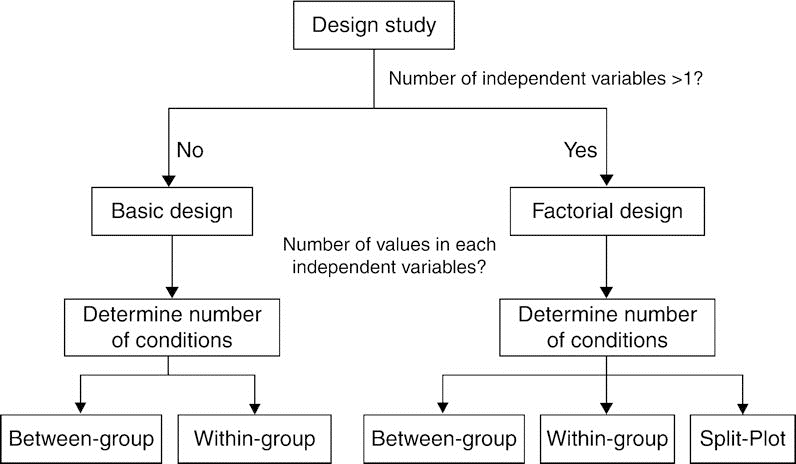
\includegraphics[scale=.5]{Hypothesis1}
\caption{Design study model}
\label{fig:designstudy}
\end{figure}

The difference between the two models is the fundamental test-structure, as seen in figure \ref{fig:designstudy}. In a between-group design, each participant is only exposed to a single experimental condition, meaning in this case he/she would only be playing the vehicle game with one of the controllers, not experiencing them both. In a within-group design each participant will utilize multiple conditions e.g. experiencing two polar opposite ways of controlling a game to establish which is the most user-friendly and convenient.

A within-group approach is usually less time-consuming due to decrease in the number of samples i.e. less test subjects needed to achieve a conclusive result \parencite{Lazar2010}.

Furthermore, Lazar argues that a Between-group construction creates a research setting where it is harder to obtain significant results, because data from different test subjects will have to be analysed under one common denominator. This indicates that a within-group construct would be preferred when choosing the strategic approach. Choosing a within-group construct is, however, not entirely without precautions.
\bigskip

\textit{Since the participants complete the same types of task under multiple conditions, they are very likely to learn from the experience and may get better in completing the tasks.}\parencite{Lazar2010}
\bigskip

This indicates that there is an increased risk of getting biased results, if user-experience is not taken into consideration. If a test subject is introduced to one control-system, and afterwards will try another as to compare the performance he/she may already be familiar with the conditions, and thus a reliable comparison cannot be substantiated. Lazar suggests changing the conditions e.g. altering the sequence of the test randomly per test subject, and furthermore changing the layout e.g. alternative racetrack can plausibly reduce the risk of getting biased samples. 


\subsubsection{Triangulation of data}
Whenever data is collected for any sort of experiment, risks of undermining the data by bias is always present. To prevent evident bias, many different approaches to minimizing the risk of bias can be initiated. 

One, more general, strategy to use, however, is that of data triangulation. The idea behind data triangulation is that by having multiple different data sets (as a result of having multiple tests) from each participant, it is possible to "precisely measure location" \parencite{Lazar2010}; 
in other words -  more accurately measure a tester's response to a product, for example.
\bigskip

An example of how triangulation can be used in practice is first by having the test subject do the experiment, while being observed. Then the test subject is asked about previous experiences (e.g. anecdotes) and their thoughts about similar products. And finally they are asked about future expectations of technology (or whatever subject is being researched).
\bigskip

From these three data sources, an overview of that tester's reaction to technology can be measured - A combination of how the person reacted during the experiment and how they responded to both the questions about past experiences and future expectations. This can give a relatively precise measure of how that person feels about a problem, compared to if they had just been handed a questionnaire, where they, themselves, should rate the product \parencite{Lazar2010}.
\bigskip

The purpose of using triangulation of data, is to minimize the risk of bias, by minimizing the risk of misinterpretation of data - just like it is hard to interpret the direction of a vector in math, from only a single point, it can be hard to interpret the intent of only a single set of data. Whereas multiple data sets (or point, in the context of vectors) will often have a more well defined "heading" (i.e. a user's reaction to a product, for example), thus making it easier to interpret accurately.

That being said, the use of triangulation does still not guarantee bias-free results, as data sources might be diverging, with the data covering different observations. When this happens, the test can still be valid, and triangulation still feasible to some extent, but it is usually not possible to reach a decisive conclusion based on such data alone, which in turn means that further testing might be required if a definitive answer to a test is needed \parencite{Lazar2010}.


\subsubsection{Usability Test}
Testing the product during development is an important aspect of any development process. Usability testing of a prototype involves the user into the testing of the product to make sure that the product is developing in the intended direction, and also determines to which degree the requirements have been proper implemented in terms of functionality. User based testing is usually used to test layouts of user interfaces and other user related aspects of the product.

\noindent Usability testing of a prototype involves \parencite{Lazar2010}:
\begin{itemize}
\item testing prototypes that have only been built on paper (known as paper prototypes);
\item testing prototypes that look complete but have a human behind the scenes responding (known as the “Wizard of Oz” technique);
\item testing working versions of software before it is officially released;
\item testing software that has already been implemented in existing systems. 

\end{itemize}


\subsubsection{Preliminary Test}
The preliminary test is a test prior to the actual test of the implemented product. The test is an examination of the specific method for which the final test is conducted. It will illuminate the different aspects in terms of procedure and results and if the designated procedures are functioning as intended. 

What will be happening, is a preliminary replica of the designated test will be conducted, where instead of having focus on the specific acquired data results, the test is the actual data, from which will be examined to account for the success of the test structure.
